\documentclass[10pt,letterpaper]{article}
\usepackage{cogsci}
\usepackage{pslatex}
\usepackage{color}
\usepackage{placeins}
\usepackage{natbib}
\usepackage{graphicx}
\usepackage{amsmath, amssymb}
\usepackage{algorithm}
\usepackage[noend]{algpseudocode}
\usepackage{amsmath,amsfonts,amsthm,amssymb}

\title{Active learning as a means to distinguish among prominent decision strategies}
\author{{\large \bf Paula Parpart (paula.parpart.10@ucl.ac.uk)}, {\large \bf Eric Schulz (eric.schulz.13@ucl.ac.uk)}, \\{\large \bf Maarten Speekenbrink (m.speekenbrink@ucl.ac.uk)} \& {\large \bf Bradley C. Love (b.love@ucl.ac.uk)}\medskip\\
Department of Experimental Psychology, University College London, London, WC1H 0AP} 


\begin{document}

\maketitle

\begin{abstract}
A long-standing debate in decision making has been whether people rely on very little information for making choices, or weigh and add all available information. We propose a new method to determine whether a non-compensatory (Take-The-Best) or compensatory strategy (Logistic Regression) is more psychologically plausible: by looking at people’s active learning queries. This method goes beyond traditional model selection techniques as it reveals the information people choose to learn early on, which subsequently drives their decisions.  We developed active learning algorithms for both Take-The-Best and Logistic Regression, and designed an active learning experiment to distinguish between these models. By letting both models and humans actively learn, we could compare their queries, and found that people follow a rank-based learning strategy in non-compensatory environments, but prefer more certainty-based queries in compensatory environments. We argue that active learning studies provide a promising new methodology to distinguish among decision models.\\ 
\medskip\\
\textbf{Keywords:} 
Decision Making, Heuristics, Active Learning, Take-The-Best
\end{abstract}

\section{Introduction}
How do we decide between two alternatives? This question is as fundamental to research in judgment and decision making as its answer is controversial \citep{todd2000precis}. Whereas some cognitive scientists believe that people only require a few pieces of information to come up with good decisions \citep{marewski2010good}, others have described humans as integrating all the evidence for both alternatives to make a decision \citep{arkes1986factors} . One of the core questions in this debate concerns the way in which people look up and integrate information.\\
Imagine you have to decide between two restaurants to go for lunch. Both restaurants differ on several binary cues (for example, one is in walkable distance, the other is not). One decision strategy you could apply is to weigh the cues by their importance and add them up; this is called a weighted additive linear model \citep[WADD]{payne1993adaptive}. For each restaurant, WADD would compute a weighted sum, and the restaurant with the larger sum is chosen. Alternatively, people might prefer a simpler strategy and base their decision only on one cue. This is what the Take-The-Best heuristic \citep[TTB]{gigerenzer1996reasoning} does: it creates a ranking order of the cues according to their validities, and chooses the restaurant that is preferred by the highest ranked cue. If that cue does not discriminate between restaurants, then the second cue is considered, and so forth. WADD is a \textit{compensatory} strategy, whereas TTB is a \textit{non-compensatory} strategy. Compensatory strategies have the property that a cue can be compensated for by combinations of subsequent cues and regression is a typical examples thereof. In contrast, the non-compensatory Take-The-Best heuristic ignores most cues to make decisions, as the most powerful cue $C_k$ can outweigh any combination of the subsequent cues $C_{k+1},\dots,C_{k+n}$ \citep{gigerenzer1999betting}. Both strategies are known to perform best in matching environments that have the same properties, i.e., WADD performs best in a compensatory environment and TTB in a non-compensatory environment \citep{martignon1999does}. 


\subsection{Traditional model testing approaches}
The dispute over the two model classes is about their psychological plausibility as models for human decision making. A repeated argument has been that non-compensatory strategies are simpler and require less computational capacity and are therefore more plausible \citep{todd2000precis}. Yet, the most common method of pitting compensatory and non-compenastory strategies against each other have been statistical simulations, showing that one outperforms the other in artificial environments. For example, multiple studies show that the simpler TTB can outperform the compensatory linear regression \citep{czerlinski1999good} in various datasets. In contrast, other studies show that there is no strong reason to prefer TTB over other cognitive models as it does not perform noticeably better \citep{chater2003fast, schulz2014predict}.\\
All of these studies argue about the predictive accuracy of cognitive models; nevertheless - just because one class of models can beat another with better predictions, it does not follow that this class is necessarily a better psychological representation of what people actually do. Although whole research paradigms are dedicated to solving the question about whether people rely on simpler non-compensatory heuristics or complex integrative mechanisms, different methodologies currently in use to answer this question are scarce and homogeneous. Another method has been probing whether participants look up additional information \citep{newell2003empirical}. This is only a limited approach to the problem at hand  since it is only ever possible to check for $k+1$ look-ups given $C_k$ cues presented so far and it has been argued that people look up additional information but do not use it \citep{marewski2011using}.\\

We propose active learning as a novel method to solve the dilemma of discriminating among compensatory and non-compensatory strategies as psychologically plausible decision models. What most of the previous studies have in common is that they study people’s decision making in static, passive and highly controlled experiments. In order to answer the crucial question about what information people hold in memory and how they look up knowledge when making decisions, we believe one has to look at an earlier stage in the process --at the stage of learning the relevant information in the first place. We argue that stronger evidence for people’s use of either TTB or a WADD strategy comes from the way people actively acquire information, i.e. cue weights and cue orders, in the respective environments. If a cognitive agent has  evolutionarily developed to prefer a certain class of models as her means to learn a cognitive representation in a particular environment, then the way she sequentially selects information should (at least partially) reflect this representation. For example, if an agent has come to apply TTB, then -intuitively- she should try to find the most important cue first as this will decrease her uncertainty maximally, and so forth. Using this way of re-creating the structure of a cognitive mechanism, it becomes possible to set up active learning algorithms for many different cognitive models over time. 

\subsection{Active Learning: Do people learn with respect to cue weights or cue orders?}
The main idea of psychological theories of active learning is to describe a learning agent as optimally designing experiments \citep{chaloner1989optimal}. That is, given that one has to find the true hypothesis out of many potential explanations as fast as possible, an agent assigns prior probabilities to each hypothesis according to some objective criterion such as the available frequency data or according to the subjectively judged plausibility of each hypothesis. Each possible outcome of any possible experiment can thus be considered, and a ``preposterior analysis'' \citep{raiffaapplied} of the ways in which each possible experimental outcome could modify beliefs about the hypothesis, can be conducted. The proposals for optimal experimental design (OED) work in an information gain-driven fashion and maximize an informational utility, which is typically a measure of how much beliefs have changed or how large the uncertainty reduction is. There has been a great deal of interest in both normative and descriptive questions surrounding human information acquisition. In a probabilistic framework, many OED models have been used to model human behavior on cognitive tasks such as feature learning \citep{griffiths2009analyzing}, reward-specific information search \citep{meder2012information}, and to assess the trade-off between exploration and exploitation \citep{knox2011nature}.\\
In this current study, we want to assess to what extent different OED models match participants' behavior in an active learning experiment, but with the goal of distinguishing among decision models. We specifically designed the perfect environments for both model classes, i.e., a fully non-compensatory environment for TTB, and a fully compensatory environment for logistic regression (WADD strategy), and several environments in between these extremes. As there are no active learning counterparts to the two decision models yet, we focus on qualitative predictions. Consequently, we developed two entropy-minimizing learning algorithms, one for a cue-ranking strategy and one for a cue-weighing strategy. Next, we compare the models' a priori search queries to the queries made by participants in an active learning task with pairwise comparisons. By letting people freely choose among pairwise comparisons, we can investigate whether people pick information such that they learn about cue orders, or instead learn cue weights directly as proposed by the active WADD strategy.

\section{Active learning algorithms}
Both active learning algorithms essentially rely on a one-step ahead greedy entropy minimization of their posterior estimates. Greedy algorithms always choose as the next observation that which currently promises to reduce the uncertainty about the learning model maximally. 


\subsection{Take-The-Best}
The active learning algorithm for the Take-The-Best heuristic is based on a greedy method that considers a distribution over all possible cue orders. Therefore, we generated all possible cue orders given the features, including those where some cues are unimportant or negatively correlated with the outcome. Putting a uniform prior over these cue orders via pseudo counts then enables us to calculate the Shannon entropy over all cue orders. All cue orders here means all TTB-like trees with possible positive and negative cue combinations that can be generated given the feature variables, including trees that only contain parts of the variables and therefore consider others as unimportant\footnote{This results in a very complex hypothesis space that increases exponentially with the number of features}. The way we assess Shannon's entropy is by establishing pseudo-counts over all cue orders and then standardizing them via the sum of all counts. Using the resulting values as a probability density distribution, our algorithm predicts new cases by generating a Take The Best output for each of the cue orders and then estimating the overall mean, weighted by every cue order's current probability. Using this approach, we can easily estimate the probability for a new test item to be a win or a loss and calculate the expected reduction in entropy over all cues given a new training item. Entropy can be reduced via some cue orders potentially generating correct predictions and thereby getting more counts ($+1$) on their pseudocounts. The used distribution over all possible cue orders can also be seen as a distribution over the whole hypothesis space. The way our algorithm then works is by the attempt to drive down the uncertainty of this hypothesis space as quickly as possible, an approach that is close to optimal in a Bayesian active learning context \citep{golovin2010near}. 
\subsection{Logistic Regression}
Logistic regression is set up as a competing compensatory model to the non-compensatory TTB model. We use a Bayesian version of logistic regression based on a random walk Metropolis MCMC algorithm. Again, the way the algorithm works is by maximizing the expected information gain for each trial. However, as a logistic regression does not learn cue orders, the expected information gain is approximated by the combined variance of all weights, the $\beta$-estimates. This means that a Bayesian logistic regression is fitted to all past observations and the current variance for all $\beta$s is calculated and then compared to the variances that could be expected from a newly fit model given a new input. This uncertainty sampling-based algorithm provides us with a compensatory active learning algorithm for the scenarios at hand. Instead of trying to drive down the hypothesis space as quickly as possible, this algorithm tries to learn about the weights as precisely as possible in order to make good compensatory judgments. 
\section{Degrees of Compensatoriness}
We are interested in the performance of the two proposed active learning models in environments with different ``compensatoriness''. Note that a non-compensatory environment can be defined as a WADD environment in which the $\beta$ weights are exponentially decreasing. In order to create different degrees of ``compensatoriness'', we make use of a mathematical trick that allows us to rely on a single parameter to smoothly vary from compensatory to non-compensatory environments through a ``stick breaking process''. The generation would be of a set of 4 weights ${\beta}_{k=1}^4$ through:

\begin{align}
\beta'_k &\sim \text{Beta}(1,\theta)\\
\text{Define}&~ \{\beta'_k\}^4_{k=1}\text{ as:}\\
\beta_k&=\beta'_k\prod_{i=1}^{k-1}(1-\beta'_i) 
\end{align}
As the expectation of the Beta-distribution is defined as $\frac{\alpha}{\alpha+\theta}$, a perfect  Take-The-Best environment corresponds to setting $\theta$ to 1 or greater as this would lead to a perfectly non-compensatory weight structure. Given the strict boarder of $\theta=1$ that separates compensatory from non-compensatory strategies, we will use $\mathbf{\theta}=[~0,0.5,1,2,\infty]$ for all the upcoming scenarios as this generates degrees of compensatoriness starting from uniform weights ($\theta=0$) all the way to an environment where only one cue matters ($\theta=\infty$). Figure~\ref{comp} shows the weighting structures that result from simulating different levels of compensatoriness for four cues by increasing $\theta$.  
\begin{figure}[htb!]
  \centering
    \caption{Compensatoriness for five different levels of $\theta$. The x-axis represents four different cues and the y-axis displays the weight magnitudes.}
\label{comp}
    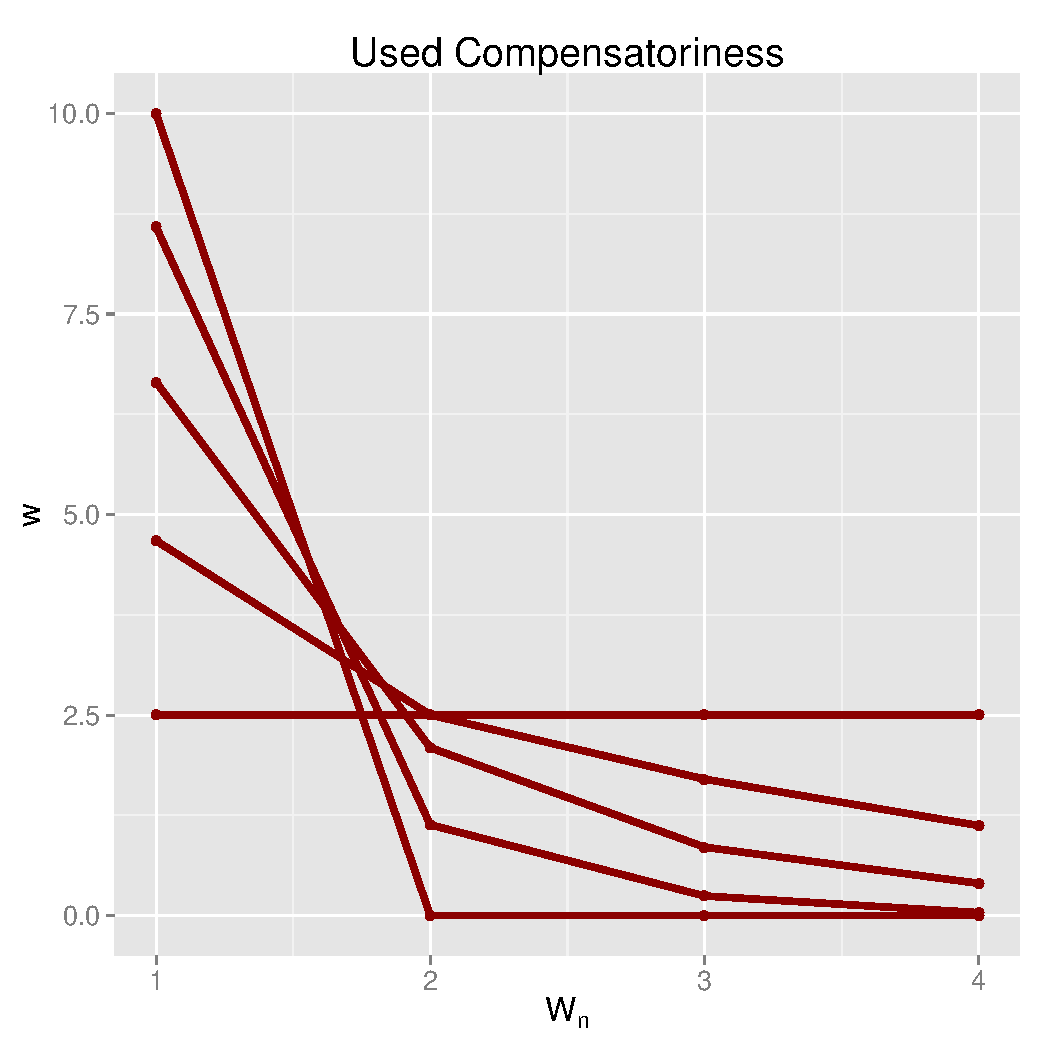
\includegraphics[scale=0.4]{comp.pdf}

\end{figure}
\noindent

\section{Experiment}
The experiment was designed to find out whether people are more likely to follow a rank-based or a weight –based active learning algorithm. The outcome has strong implications for either decision mechanism as plausible decision strategies. We hypothesized that people are sensitive to the structure of the environment (the degree of compensatoriness) in their choice of learning algorithms. We assigned people randomly to one of the five above-mentioned compensatoriness conditions. We expected participants in the more non-compensatory environments to be better matched by the active Take-The-Best algorithm, while logistic regression would better match their choices in the compensatory environments.   

\subsection{Participants}
Two hundred and sixty-four (\textit{N} = 264) participants (\textit{M} = 35.4 years) were recruited via Amazon Mechanical Turk to take part in the ``Alien Olympics" study. Participants were paid \$0.50 for participation plus an additional bonus between \$0 and  \$0.5 depending on their performance. 
\subsection{Materials and Stimuli}
On each trial, participants had to choose a pair of Aliens to compete against each other, in order to learn about their strengths. The Aliens varied on four different features, which are displayed in Figure~\ref{Alien_features}. The features were designed to be helpful in fights, e.g., wings enabled an Alien to fly which helps in attacking enemies, while camouflage is useful for defense. The features were explained to participants at the start and they were told that the different characteristics might not all be of equal importance for an Alien's strength in a fight. As there are four features, we generated all possible feature combinations which results in 16 different Alien types. On each trial, participants were presented with four random Aliens on the screen, and had to choose two of these to compete against each other. After selecting a pair, they received feedback about which Alien had won the competition. They were also told that sometimes a weaker Alien could win against a stronger competitor as in any sport, which reflects the probabilistic generation of the actual outcomes. The underlying weights of the four features that people could learn depended on the compensatoriness condition a participant was in. Importantly, we emphasized that people should pick their Aliens wisely by selecting informative comparisons out of the presented Aliens, as the goal was to learn how the different features influenced an Aliens chances to win. Participants were informed that they would need this feature knowledge later in the experiment for an assessment task. The actual outcomes observed in feedback were generated by using the weights from the respective compensatoriness conditions (standardized to always add up to 10) and applying logistic regression in order to determine an Alien's strength, or likelihood of winning against another Alien. 

\subsection{Procedure}
The experiment was divided into a learning phase and a test phase. The learning phase consisted of participants actively choosing Alien pairs to fight against each other on 30 trials. The test phase was designed to assess what people learned and was structured as follows: On each trial, participants were presented with only 2 different Aliens that were again randomly drawn from the Alien database. We told participants that these Aliens were the candidates for their Olympic Team, and it was their task to choose the Alien they considered to be stronger based on what they had learned about the characteristics. This assessment phase consisted of 10 binary choices. Participants were reminded that a bonus payment would depend on their performance in this test phase.
\begin{figure}[htb!]
		\centering
	\caption{Aliens varied on 4 different features (A-D): Antennae, Wings, Diamonds, and Camouflage. E: Alien without features, F: Alien with all features.}
	\label{Alien_features}
		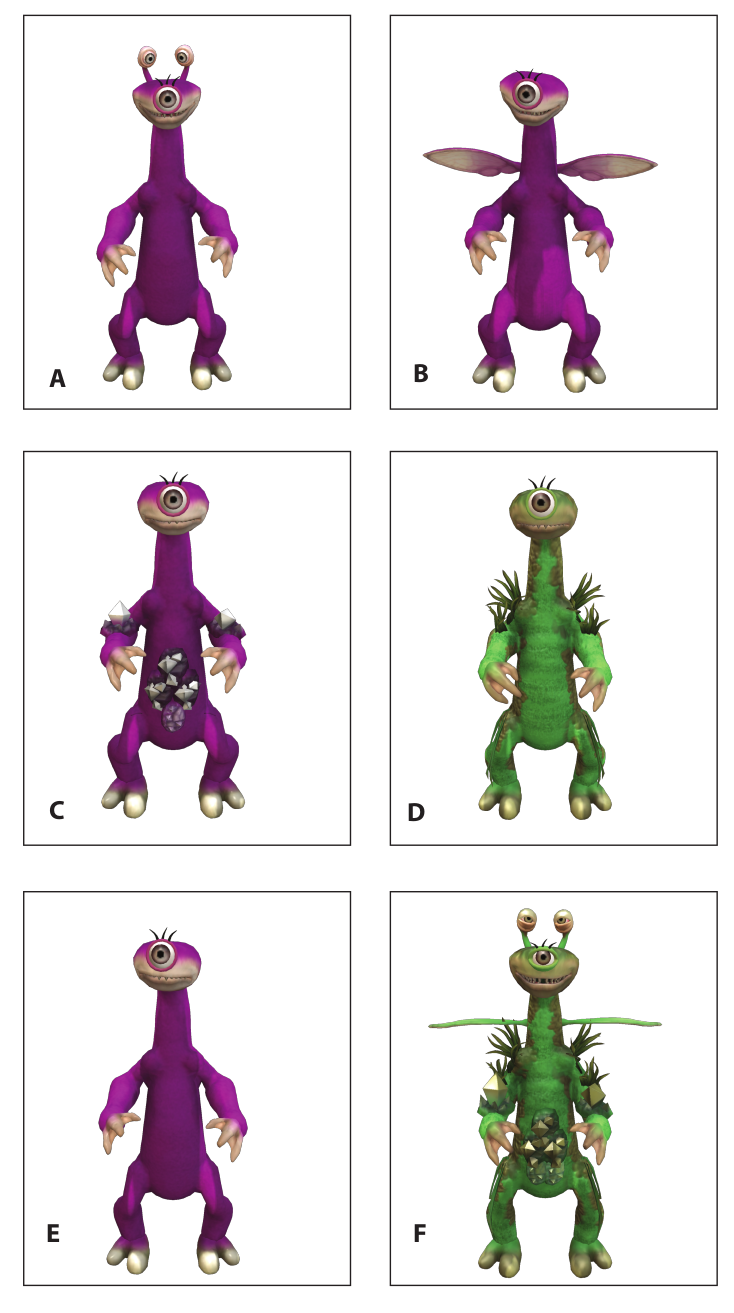
\includegraphics[scale=0.3]{aliens.png}
\end{figure}

\subsection{Results}
Participants' performance at identifying the stronger Aliens during the test stage was highly above chance; the average percentage of correct choices made was 74\% ($t(263) = 27.44,~p< 0.001$) with a range of (30\%,97\%). Performance varied as a function of the compensatoriness condition that participants were in. Figure~\ref{performance} represents the average score as a function of compensatoriness: as the environmental structure gets more non-compensatory (i.e. more weight on just a few cues), the average performance drops. This intuitively makes sense as there is less information to be learned when a cue dominates all others, which makes draws more likely and informative comparisons less likely.  However, peak performance was observed for an environment not completely compensatory ($\theta=0$), but slightly compensatory.
 
\begin{figure}[htb!]
	\centering
\caption{Average test performance across participants by compensatoriness conditions.}
	\label{performance}
	\centering
	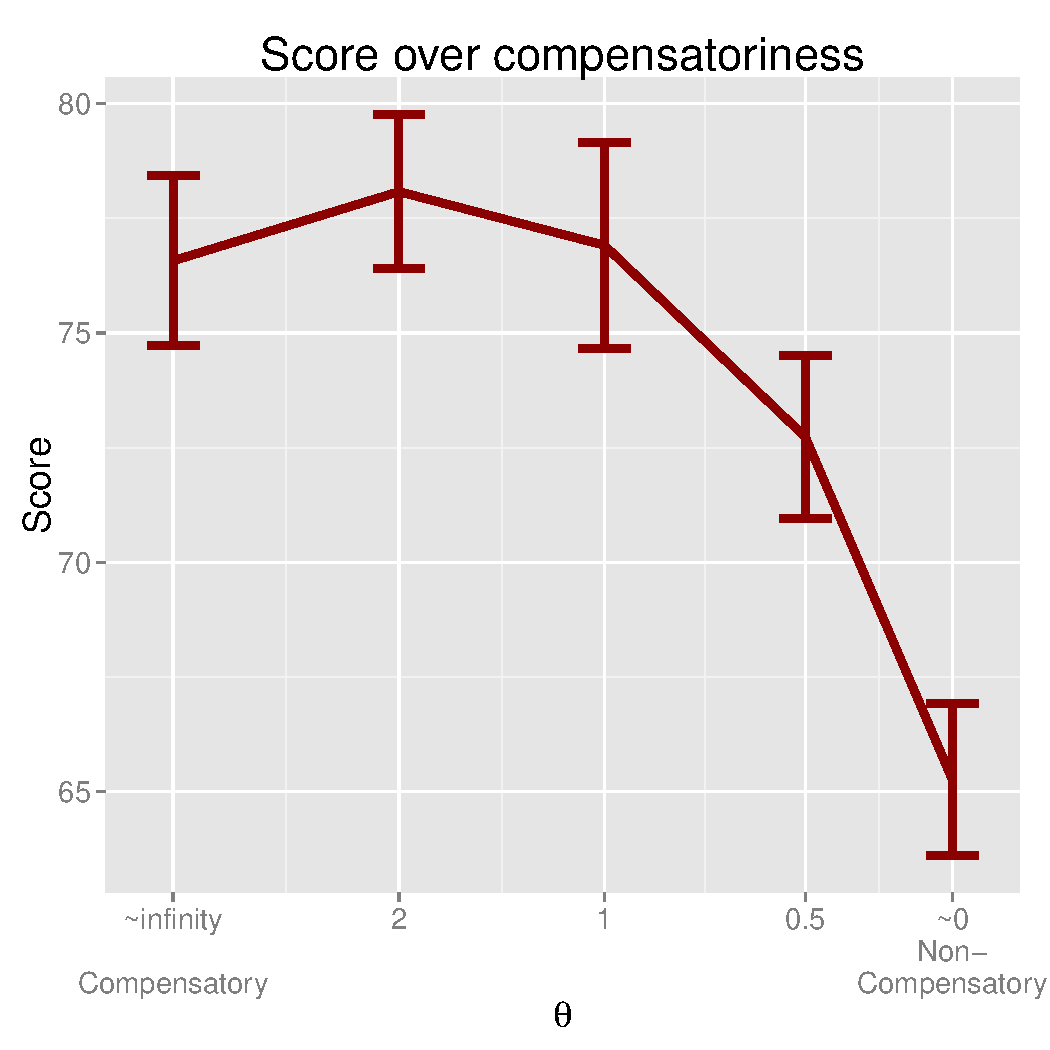
\includegraphics[scale=0.4]{score.pdf}
	
\end{figure}
\begin{figure}[htb!]
	\centering
			\caption{Behavioral model fits of the Take-the-Best Heuristic and Logistic Regression. The y-axis represents the percentage of correct predictions with respect to people's choices at test.}
	\label{percentage}
	\centering
	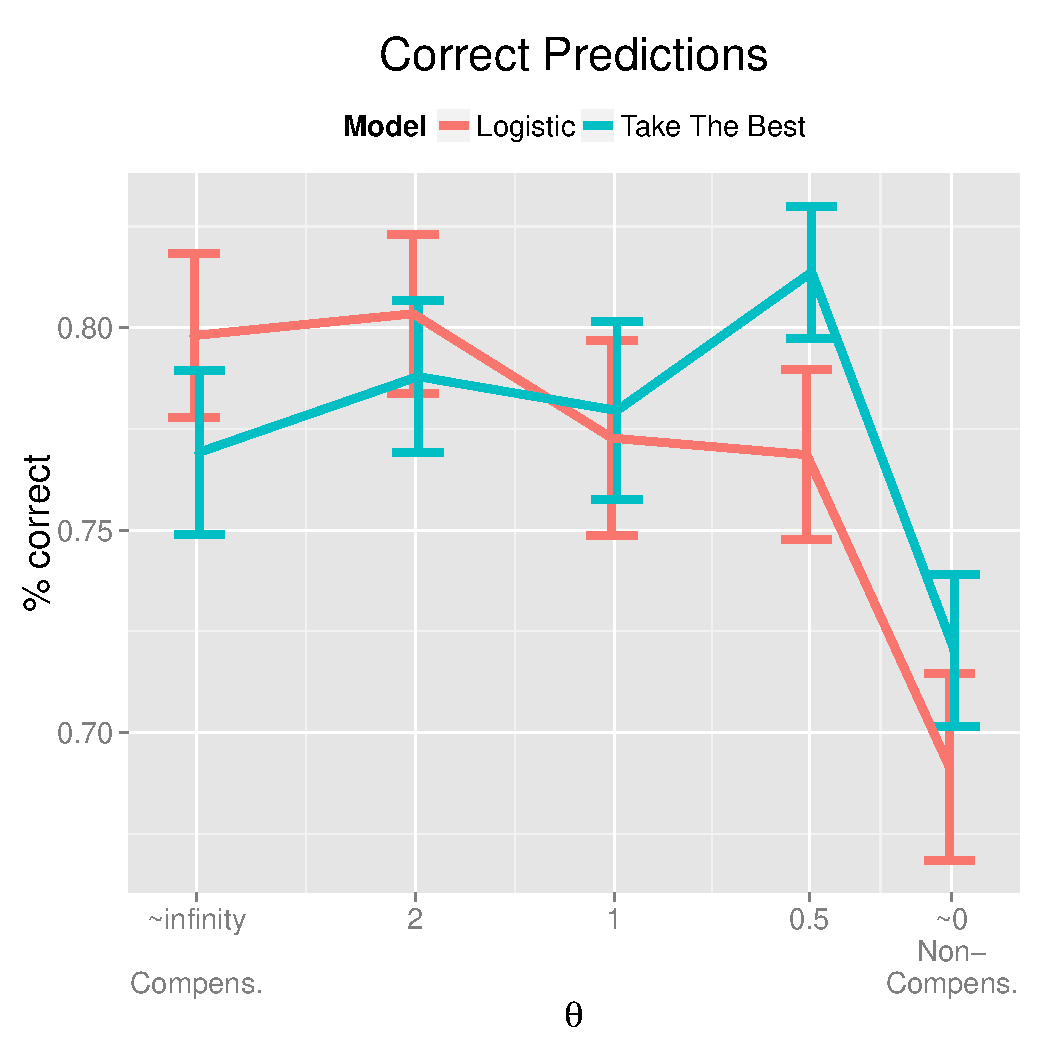
\includegraphics[scale=0.4]{percentage.pdf}

\end{figure}

Next, we demonstrate the model fits of the regular Take-The-Best heuristic and Logistic Regression to participants' choices at test. These were generated by fitting both models to the set of Aliens participants had selected, and using the fitted models to predict choices in the test set. Figure~\ref{percentage} presents the model fits as a function of the compensatoriness.  It can be seen that Take-The-Best was better at predicting people's behavior in the highly non-compensatory conditions,  whereas in the more compensatory conditions no significant difference between the models could be found. This demonstrates again that purely behavioral model fits are limited in their ability to distinguish between common decision models, even in a prediction-based test. Therefore, we focus on the active learning results next.\\
\subsubsection*{Active Learning Results}
We categorized all possible pairwise comparisons people could choose on each trial into the 8 possible subtypes that can be seen on the x-axis of Figure~\ref{shortoverview}. WDDD for example signifies a comparison of two Aliens with 3 similar features (D for draw), where one of the Aliens had one more feature than the other (W for Win). A WLDD comparison compares two Aliens with an equal direction of two features but differing in two others (W for Win, L for Loss), i.e., this might test whether the feature Wings are more important than Camouflage for the outcome.
\begin{figure}[htb!]
	\caption{The 8 subtypes of active learning choices that participants made and the a priori model choices.}
	\label{shortoverview}
	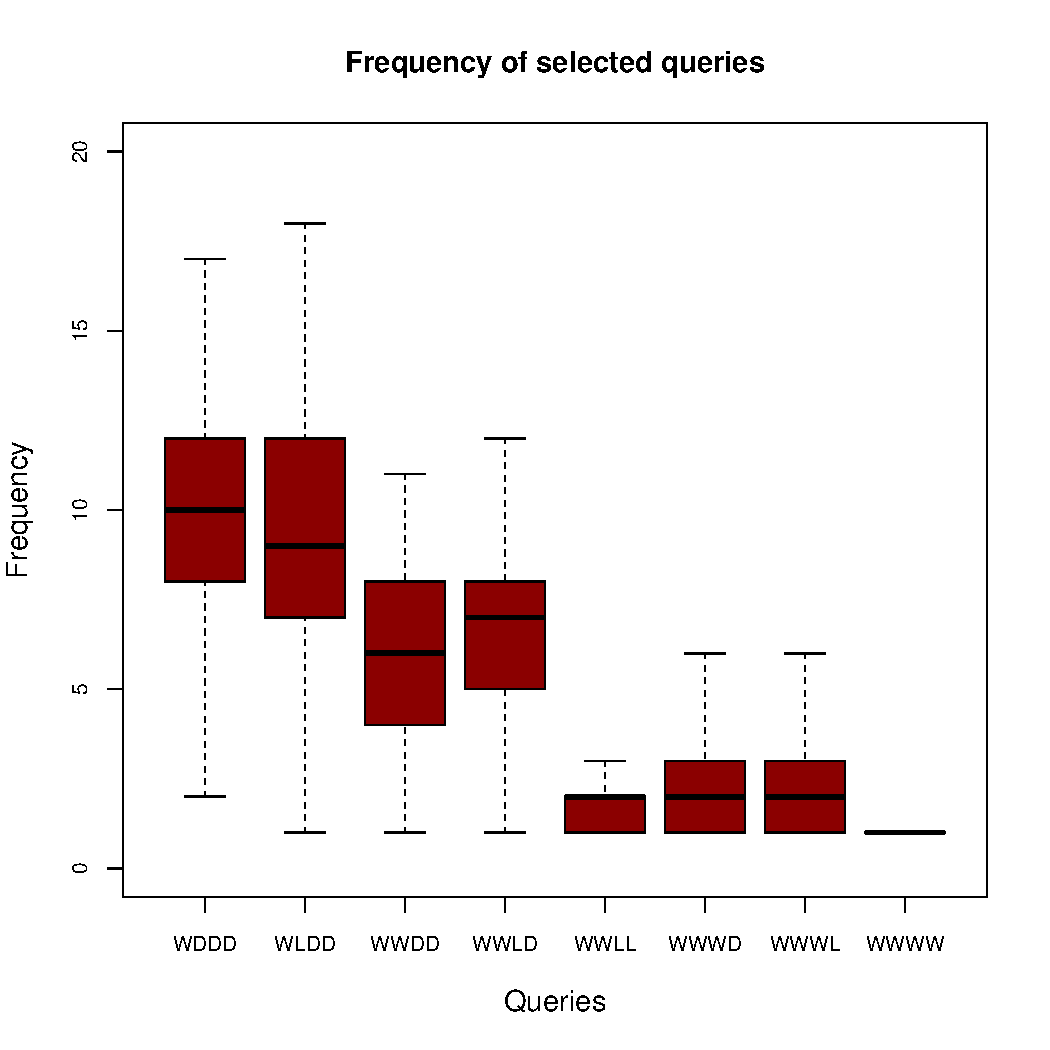
\includegraphics[scale=0.53]{shortoverview.pdf}
\end{figure}
People rarely chose comparisons where it is unclear what feature was responsible for an outcome, e.g., a  comparison of an Alien with 3 or 4 more features than its competitor (WWWD, WWWW). Instead, the most common comparisons were simpler and controlled, such as the WLDD, which test for the relative effect of one feature in comparison to another, i.e. searching for orders among features. Although participants were told in the instructions that all features are helpful in fights, the most frequent comparison was the WDDD query, assessing whether a feature improves the outcome. The fact that people preferred these simple queries could reflect a preference to perform confirmatory tests \citep{markant2012one}. Finally, we compared queries selected by the two learning algorithms against queries chosen by participants. We let both the TTB and Logistic Regression algorithms learn in the same compensatory and non-compensatory environment as the participants, by creating as many simulated participant profiles as there were participants in each compensatoriness condition. Then, we let the models learn over time. As a result, the frequencies of selections executed at each run by the algorithms were matched with those by humans and an overall correlation between the frequencies was calculated. Figure~\ref{result} shows in the lower panel how well the selection frequency predicted, and in the upper panel how well the selection frequencies by the models correlated with participants' frequencies.
\begin{figure}[htb!]
	\centering
\caption{Frequency of queries by active learning algorithms matched to participants' queries. Lower panel:  y-axis shows the variance explained. Upper panel: y-axis displays correlations.}
	\label{result}
	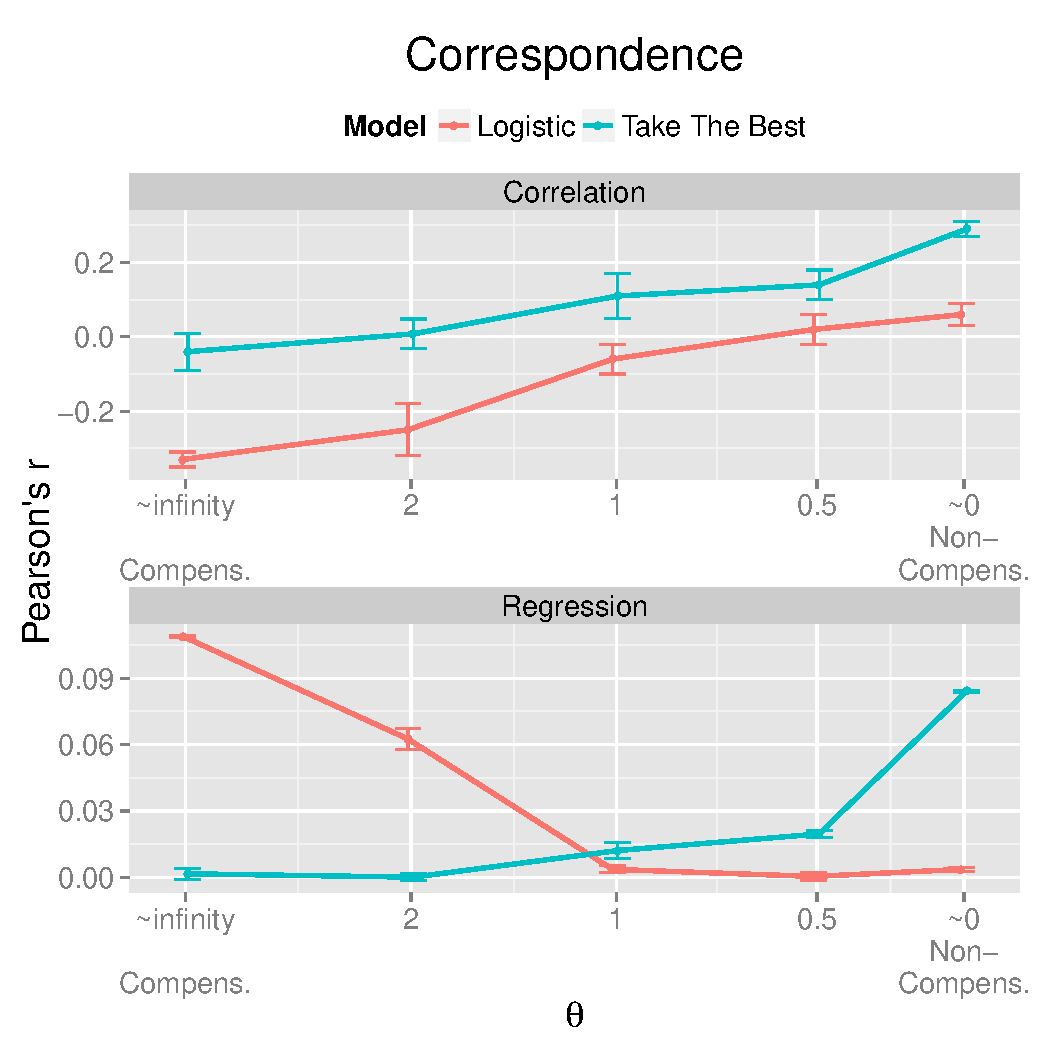
\includegraphics[scale=0.5]{results.pdf}
	
\end{figure}
 These results demonstrate that participants in different conditions differed in terms of which active learning algorithm best described their queries (lower panel, Figure~\ref{result}).  With an increase in non-compensatoriness, the Active Take-The-Best model explained more variance and Logistic Regression less, in line with our prediction. This is also reflected in the number of noncompensatory tests performed (e.g., WWLD), which increased in more non-compensatory conditions. The underlying correlations between the models' and peoples' selections (upper panel, Figure~\ref{result}) reveal a similar picture for the TTB learning algorithm - with more non-compensatoriness, the TTB algorithm's queries better matched what queries people were choosing. However, as the environment becomes more and more compensatory, participants tend to select observations that do not reduce uncertainty maximally with respect to the weight-based logistic regression algorithm, and instead select comparisons that are more certain which could reflect more confirmatory hypothesis testing. This finding also remained the same when we used predictive uncertainty instead of information gain, showing that -as environments get more compensatory- participants tend to select queries where they already know the outcome better. Overall, the Take-The-Best active learning algorithm which minimizes uncertainty with respect to cue orders was a better description of how people learn in our experiment.
\section{Discussion and Conclusion}
Results demonstrated that--at least in more non-compensatory environments-- people learn more like an order-based strategy, which lends support to the Take-The-Best heuristic as a plausible decision mechanism in these environments. This finding represents more processing-based evidence than the usual predictive accuracy findings or descriptive model fits.  Furthermore, people do seem to be adaptive in their choice of active learning strategies to the structure of the environment: the more non-compensatory the environment was, the more choices people made in accordance with the TTB active algorithm. People were not well-described by the weight-based logistic regression algorithm, and for very compensatory environments they even seemed to pick the opposite choices to the uncertainty reducing algorithm, i.e., they chose more certain queries. This could in turn be due to the fact that --when all cues are equally important-- people notice they cannot learn any cue rank orders, and so they might apply another strategy that is compensatory but not captured by logistic regression, for example a tallying strategy. This is a question we plan to address in a follow up study.\\

The current experiment demonstrates that active learning experiments can be used to distinguish among prominent decision strategies. Our results revealed a more informative picture than the traditional passive model fitting procedures. We believe that the application of active learning algorithms as a means to distinguish among decision algorithms is a novel and promising approach. Creating active versions of classic decision models and testing them in related experiments will shed more light onto how people actually learn in different tasks. We hope to utilize this new approach for more process-based comparisons between different learning and decision making models in the near future.
\section{Acknowledgements}
PP and ES contributed equally. They are both supported by the UK Centre for Doctoral Training in Financial Computing \& Analytics.  This work is partly supported by the Leverhulme Trust grant RPG-2014-075 to BCL. An appendix explaining the computational models in more detail can be found at: https://github.com/ericschulz/activemodeltest.
\footnotesize
\bibliographystyle{apa-good}
\bibliography{Bibo}
\end{document}
